\documentclass{ximera}

%\usepackage{todonotes}

\newcommand{\todo}{}

\usepackage{esint} % for \oiint
\ifxake%%https://math.meta.stackexchange.com/questions/9973/how-do-you-render-a-closed-surface-double-integral
\renewcommand{\oiint}{{\large\bigcirc}\kern-1.56em\iint}
\fi


\graphicspath{
  {./}
  {ximeraTutorial/}
  {basicPhilosophy/}
  {functionsOfSeveralVariables/}
  {normalVectors/}
  {lagrangeMultipliers/}
  {vectorFields/}
  {greensTheorem/}
  {shapeOfThingsToCome/}
  {dotProducts/}
  {partialDerivativesAndTheGradientVector/}
  {../productAndQuotientRules/exercises/}
  {../normalVectors/exercisesParametricPlots/}
  {../continuityOfFunctionsOfSeveralVariables/exercises/}
  {../partialDerivativesAndTheGradientVector/exercises/}
  {../directionalDerivativeAndChainRule/exercises/}
  {../commonCoordinates/exercisesCylindricalCoordinates/}
  {../commonCoordinates/exercisesSphericalCoordinates/}
  {../greensTheorem/exercisesCurlAndLineIntegrals/}
  {../greensTheorem/exercisesDivergenceAndLineIntegrals/}
  {../shapeOfThingsToCome/exercisesDivergenceTheorem/}
  {../greensTheorem/}
  {../shapeOfThingsToCome/}
  {../separableDifferentialEquations/exercises/}
  {vectorFields/}
}

\newcommand{\mooculus}{\textsf{\textbf{MOOC}\textnormal{\textsf{ULUS}}}}

\usepackage{tkz-euclide}
\usepackage{tikz}
\usepackage{tikz-cd}
\usetikzlibrary{arrows}
\tikzset{>=stealth,commutative diagrams/.cd,
  arrow style=tikz,diagrams={>=stealth}} %% cool arrow head
\tikzset{shorten <>/.style={ shorten >=#1, shorten <=#1 } } %% allows shorter vectors

\usetikzlibrary{backgrounds} %% for boxes around graphs
\usetikzlibrary{shapes,positioning}  %% Clouds and stars
\usetikzlibrary{matrix} %% for matrix
\usepgfplotslibrary{polar} %% for polar plots
\usepgfplotslibrary{fillbetween} %% to shade area between curves in TikZ
%\usetkzobj{all}
\usepackage[makeroom]{cancel} %% for strike outs
%\usepackage{mathtools} %% for pretty underbrace % Breaks Ximera
%\usepackage{multicol}
\usepackage{pgffor} %% required for integral for loops



%% http://tex.stackexchange.com/questions/66490/drawing-a-tikz-arc-specifying-the-center
%% Draws beach ball
\tikzset{pics/carc/.style args={#1:#2:#3}{code={\draw[pic actions] (#1:#3) arc(#1:#2:#3);}}}



\usepackage{array}
\setlength{\extrarowheight}{+.1cm}
\newdimen\digitwidth
\settowidth\digitwidth{9}
\def\divrule#1#2{
\noalign{\moveright#1\digitwidth
\vbox{\hrule width#2\digitwidth}}}




% \newcommand{\RR}{\mathbb R}
% \newcommand{\R}{\mathbb R}
% \newcommand{\N}{\mathbb N}
% \newcommand{\Z}{\mathbb Z}

\newcommand{\sagemath}{\textsf{SageMath}}


%\renewcommand{\d}{\,d\!}
%\renewcommand{\d}{\mathop{}\!d}
%\newcommand{\dd}[2][]{\frac{\d #1}{\d #2}}
%\newcommand{\pp}[2][]{\frac{\partial #1}{\partial #2}}
% \renewcommand{\l}{\ell}
%\newcommand{\ddx}{\frac{d}{\d x}}

% \newcommand{\zeroOverZero}{\ensuremath{\boldsymbol{\tfrac{0}{0}}}}
%\newcommand{\inftyOverInfty}{\ensuremath{\boldsymbol{\tfrac{\infty}{\infty}}}}
%\newcommand{\zeroOverInfty}{\ensuremath{\boldsymbol{\tfrac{0}{\infty}}}}
%\newcommand{\zeroTimesInfty}{\ensuremath{\small\boldsymbol{0\cdot \infty}}}
%\newcommand{\inftyMinusInfty}{\ensuremath{\small\boldsymbol{\infty - \infty}}}
%\newcommand{\oneToInfty}{\ensuremath{\boldsymbol{1^\infty}}}
%\newcommand{\zeroToZero}{\ensuremath{\boldsymbol{0^0}}}
%\newcommand{\inftyToZero}{\ensuremath{\boldsymbol{\infty^0}}}



% \newcommand{\numOverZero}{\ensuremath{\boldsymbol{\tfrac{\#}{0}}}}
% \newcommand{\dfn}{\textbf}
% \newcommand{\unit}{\,\mathrm}
% \newcommand{\unit}{\mathop{}\!\mathrm}
% \newcommand{\eval}[1]{\bigg[ #1 \bigg]}
% \newcommand{\seq}[1]{\left( #1 \right)}
% \renewcommand{\epsilon}{\varepsilon}
% \renewcommand{\phi}{\varphi}


% \renewcommand{\iff}{\Leftrightarrow}

% \DeclareMathOperator{\arccot}{arccot}
% \DeclareMathOperator{\arcsec}{arcsec}
% \DeclareMathOperator{\arccsc}{arccsc}
% \DeclareMathOperator{\si}{Si}
% \DeclareMathOperator{\scal}{scal}
% \DeclareMathOperator{\sign}{sign}


%% \newcommand{\tightoverset}[2]{% for arrow vec
%%   \mathop{#2}\limits^{\vbox to -.5ex{\kern-0.75ex\hbox{$#1$}\vss}}}
% \newcommand{\arrowvec}[1]{{\overset{\rightharpoonup}{#1}}}
% \renewcommand{\vec}[1]{\arrowvec{\mathbf{#1}}}
% \renewcommand{\vec}[1]{{\overset{\boldsymbol{\rightharpoonup}}{\mathbf{#1}}}}

% \newcommand{\point}[1]{\left(#1\right)} %this allows \vector{ to be changed to \vector{ with a quick find and replace
% \newcommand{\pt}[1]{\mathbf{#1}} %this allows \vec{ to be changed to \vec{ with a quick find and replace
% \newcommand{\Lim}[2]{\lim_{\point{#1} \to \point{#2}}} %Bart, I changed this to point since I want to use it.  It runs through both of the exercise and exerciseE files in limits section, which is why it was in each document to start with.

% \DeclareMathOperator{\proj}{\mathbf{proj}}
% \newcommand{\veci}{{\boldsymbol{\hat{\imath}}}}
% \newcommand{\vecj}{{\boldsymbol{\hat{\jmath}}}}
% \newcommand{\veck}{{\boldsymbol{\hat{k}}}}
% \newcommand{\vecl}{\vec{\boldsymbol{\l}}}
% \newcommand{\uvec}[1]{\mathbf{\hat{#1}}}
% \newcommand{\utan}{\mathbf{\hat{t}}}
% \newcommand{\unormal}{\mathbf{\hat{n}}}
% \newcommand{\ubinormal}{\mathbf{\hat{b}}}

% \newcommand{\dotp}{\bullet}
% \newcommand{\cross}{\boldsymbol\times}
% \newcommand{\grad}{\boldsymbol\nabla}
% \newcommand{\divergence}{\grad\dotp}
% \newcommand{\curl}{\grad\cross}
%\DeclareMathOperator{\divergence}{divergence}
%\DeclareMathOperator{\curl}[1]{\grad\cross #1}
% \newcommand{\lto}{\mathop{\longrightarrow\,}\limits}

% \renewcommand{\bar}{\overline}

\colorlet{textColor}{black}
\colorlet{background}{white}
\colorlet{penColor}{blue!50!black} % Color of a curve in a plot
\colorlet{penColor2}{red!50!black}% Color of a curve in a plot
\colorlet{penColor3}{red!50!blue} % Color of a curve in a plot
\colorlet{penColor4}{green!50!black} % Color of a curve in a plot
\colorlet{penColor5}{orange!80!black} % Color of a curve in a plot
\colorlet{penColor6}{yellow!70!black} % Color of a curve in a plot
\colorlet{fill1}{penColor!20} % Color of fill in a plot
\colorlet{fill2}{penColor2!20} % Color of fill in a plot
\colorlet{fillp}{fill1} % Color of positive area
\colorlet{filln}{penColor2!20} % Color of negative area
\colorlet{fill3}{penColor3!20} % Fill
\colorlet{fill4}{penColor4!20} % Fill
\colorlet{fill5}{penColor5!20} % Fill
\colorlet{gridColor}{gray!50} % Color of grid in a plot

\newcommand{\surfaceColor}{violet}
\newcommand{\surfaceColorTwo}{redyellow}
\newcommand{\sliceColor}{greenyellow}




\pgfmathdeclarefunction{gauss}{2}{% gives gaussian
  \pgfmathparse{1/(#2*sqrt(2*pi))*exp(-((x-#1)^2)/(2*#2^2))}%
}


%%%%%%%%%%%%%
%% Vectors
%%%%%%%%%%%%%

%% Simple horiz vectors
\renewcommand{\vector}[1]{\left\langle #1\right\rangle}


%% %% Complex Horiz Vectors with angle brackets
%% \makeatletter
%% \renewcommand{\vector}[2][ , ]{\left\langle%
%%   \def\nextitem{\def\nextitem{#1}}%
%%   \@for \el:=#2\do{\nextitem\el}\right\rangle%
%% }
%% \makeatother

%% %% Vertical Vectors
%% \def\vector#1{\begin{bmatrix}\vecListA#1,,\end{bmatrix}}
%% \def\vecListA#1,{\if,#1,\else #1\cr \expandafter \vecListA \fi}

%%%%%%%%%%%%%
%% End of vectors
%%%%%%%%%%%%%

%\newcommand{\fullwidth}{}
%\newcommand{\normalwidth}{}



%% makes a snazzy t-chart for evaluating functions
%\newenvironment{tchart}{\rowcolors{2}{}{background!90!textColor}\array}{\endarray}

%%This is to help with formatting on future title pages.
\newenvironment{sectionOutcomes}{}{}



%% Flowchart stuff
%\tikzstyle{startstop} = [rectangle, rounded corners, minimum width=3cm, minimum height=1cm,text centered, draw=black]
%\tikzstyle{question} = [rectangle, minimum width=3cm, minimum height=1cm, text centered, draw=black]
%\tikzstyle{decision} = [trapezium, trapezium left angle=70, trapezium right angle=110, minimum width=3cm, minimum height=1cm, text centered, draw=black]
%\tikzstyle{question} = [rectangle, rounded corners, minimum width=3cm, minimum height=1cm,text centered, draw=black]
%\tikzstyle{process} = [rectangle, minimum width=3cm, minimum height=1cm, text centered, draw=black]
%\tikzstyle{decision} = [trapezium, trapezium left angle=70, trapezium right angle=110, minimum width=3cm, minimum height=1cm, text centered, draw=black]


\title{Analysis}

\begin{document}

\begin{abstract}
8 characteristics
\end{abstract}
\maketitle





\section*{Linear Function Analysis}

What do we want to know when we analyze any function?

We want to know the 
\begin{itemize}
     \item \textbf{\textcolor{red!70!black}{Domain}} 
     \item \textbf{\textcolor{red!70!black}{Zeros}} 
     \item \textbf{\textcolor{red!70!black}{Continuity}} 
\begin{itemize}
     \item \textbf{\textcolor{purple!85!blue}{discontinuities}} 
     \item \textbf{\textcolor{purple!85!blue}{singularities}} 
\end{itemize}
     \item \textbf{\textcolor{red!70!black}{End-Behavior}} 
     \item \textbf{\textcolor{red!70!black}{Behavior}} 
\begin{itemize}
     \item \textbf{\textcolor{purple!85!blue}{intervals where increasing}} 
     \item \textbf{\textcolor{purple!85!blue}{intervals where decreasing}} 
\end{itemize}
     \item \textbf{\textcolor{red!70!black}{Global Maximum and Minimum}} 
     \item \textbf{\textcolor{red!70!black}{Local Maximums and Minimums}} 
     \item \textbf{\textcolor{red!70!black}{Range}} 
     \item \textbf{\textcolor{blue!55!black}{...and we would like a nice graph}} 
\end{itemize}

We want all of this information for linear functions and we want exact information, not approximations. \\

Remember, we are beginning with graphical analysis, because that is a familiar jumping off point for students.  But, graphs are inherently inaccurate tools.  That isn't what we want. We are taking our familiarity with graphical descriptions and moving them over to algebraic descriptions, because algebra is our exact tool. \\

Linear functions are our initial bridge to exactness. \\


Linear functions are those functions which can be described with formulas like

\[
L(x) = A \, x + B 
\]



\begin{warning}

The leading coefficient, $A$, can be $0$ in our template for linear functions. \\

\[
L(x) = B 
\]

In this case, the linear function is a constant function.  Constant functions are special types of linear functions. Their graphs are lines, like the graphs of all linear functions.  They are just horizontal lines.

\end{warning}




\subsection*{Domain} 

All linear functions are defined for all real numbers.  Their natural domain is $\mathbb{R} = (-\infty, \infty)$. \\

If you can identify a function as linear, then you automatically know its domain. \\


\textbf{Note:}  We can restrict the domain of any function.  Restricting the domain just means that the stated domain is not all of the numbers that could be used in the formula.  For linear functions, we will alert the reader by titling such functions as restricted linear functions.\\







\subsection*{Zeros}

Every time we describe a characteristic for a linear function, we must separate constant functions from other linear functions. \\

Constant functions do not have zeros, unless the constant function is the zero function.  In that case every number in the domain is a zero of the function. \\


Otherwise, linear functions have exactly one zero. \\

The zero of $L(x) = A \, x + B $ is $\frac{-B}{A}$












\subsection*{Continuity}

Linear functions are continuous functions.  They have no discontinuities or singularities. \\






\subsection*{End-Behavior}


Again, if the linear function is a constant function, then the end-behavior is just that constant. \\



Otherwise, linear functions have opposite end-behavior on either side of the domain, which is given by the sign of the leading coefficient. \\


\begin{itemize}
     \item If the leading coefficient is positive,
     \begin{itemize}
          \item the function is unbounded negatively in the negative tail of the domain.
          \item the function is unbounded positively in the positive tail of the domain.
     \end{itemize}
     \item If the leading coefficient is negative,
     \begin{itemize}
          \item the function is unbounded positively in the negative tail of the domain.
          \item the function is unbounded negatively in the positive tail of the domain.
     \end{itemize}
\end{itemize}


This is probably easier to see, then write.



\begin{image}
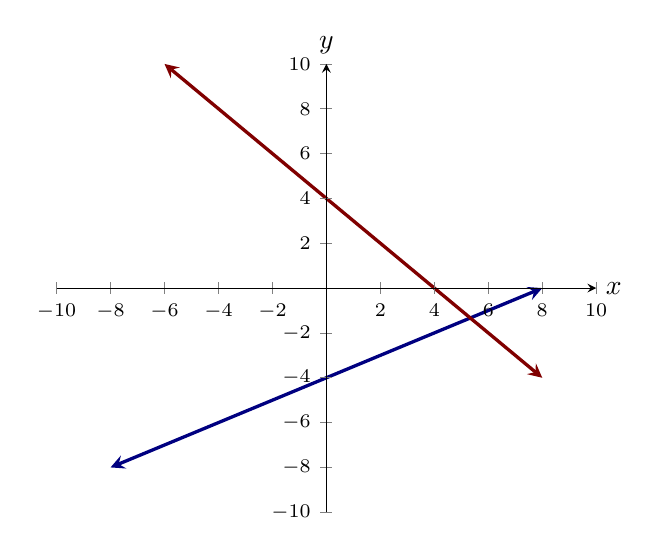
\begin{tikzpicture}
     \begin{axis}[
               domain=-10:10, ymax=10, xmax=10, ymin=-10, xmin=-10,
               axis lines =center, xlabel=$x$, ylabel=$y$, 
                ytick={-10,-8,-6,-4,-2,2,4,6,8,10}, 
                xtick={-10,-8,-6,-4,-2,2,4,6,8,10},
                ticklabel style={font=\scriptsize},
               every axis y label/.style={at=(current axis.above origin),anchor=south},
               every axis x label/.style={at=(current axis.right of origin),anchor=west},
               axis on top,
                    ]

        
        \addplot [draw=penColor, very thick, smooth, domain=(-8:8),<->] {0.5*x-4};
        \addplot [draw=penColor2, very thick, smooth, domain=(-6:8),<->] {-x+4};
        %\addplot[color=penColor,fill=penColor,only marks,mark=*] coordinates{(5.333,-1.333)};


    \end{axis}
\end{tikzpicture}
\end{image}


We will need some symbols and notation to make it easier to write about end-behavior. \\



\begin{notation}  \textbf{\textcolor{red!70!black}{A Peek Ahead}}

Our notation for end-behavior will be called \textit{limit notation}. \\



\textbf{\textcolor{blue!55!black}{$\blacktriangleright$}} the function is unbounded negatively in the negative tail of the domain.

\[
\lim\limits_{x \to -\infty} f(x) = -\infty
\]


\textbf{\textcolor{blue!55!black}{$\blacktriangleright$}} the function is unbounded positively in the positive tail of the domain.

\[
\lim\limits_{x \to \infty} f(x) = \infty
\]


\textbf{\textcolor{blue!55!black}{$\blacktriangleright$}} the function is unbounded positively in the negative tail of the domain.

\[
\lim\limits_{x \to -\infty} f(x) = \infty
\]


\textbf{\textcolor{blue!55!black}{$\blacktriangleright$}} the function is unbounded negatively in the positive tail of the domain.

\[
\lim\limits_{x \to \infty} f(x) = -\infty
\]


\end{notation}
















\subsection*{Behavior}



\textbf{\textcolor{blue!55!black}{Increasing and Decreasing}}






The graph above vividly suggests that linear functions are always increasing or always decreasing.


\begin{itemize}
\item If the leading coefficient is positive, (then the graph moves up to the right) then the linear function is an increasing function.

\item If the leading coefficient is negative, (then the graph moves down to the right) then the linear function is a decreasing function.
\end{itemize}





Increasing and decreasing refer to the rate of change.


\begin{itemize}
\item Increasing is a positive rate of change. (The domain and function values change in the same way.)
\item Decreasing is a negative rate of change. (The domain and function values change in the opposite way.)
\end{itemize}
















\subsection*{Maximums and Minimums}

\textbf{\textcolor{blue!55!black}{Global and Local}} \\
\textbf{\textcolor{blue!55!black}{Absolute and Relative}} \\


\begin{itemize}
     \item Linear functions do not have global maximums or minimums. 
     \item Linear functions do not have local maximums or minimums. 
\end{itemize}


If we restrict the domain, then we might have a maximum or minimum. \\



\begin{warning}

This is all true if the linear function is not a constant function. \\


If the linear function is a constant function, then the function only has one function value at every domain number.  That makes the one function value a global and local maximum that occurs at every domain number. \\

Weirdly enough, that also makes the one function value a global and local minimum that occurs at every domain number.

\end{warning}



\subsection*{Range}


If the linear function is a constant function, then the range is just a single number $\{ B \}$. \\

Otherwise, all linear function have the same range, $(-\infty, \infty)$ \\

\textbf{Note:} Restricting the domain will also restrict the range.\\










\begin{example}

Analyze $L(x) = 3 \, x - 5$  \\


$L(x) = 3 \, x - 5$ matches the template for a linear function $L(x) = A \, x + B$.\\
Since the leading coefficient is not $0$, $L$ is a nonconstant linear function.\\



\textbf{Domain} \\

As a linear function, the domain of $L$ is $(-\infty, \infty)$.\\


\textbf{Zeros} \\

As a nonconstant linear function, $L$ has a single zero.\\

$L(x) = 3 \, x - 5 = 0$ when $x = \frac{5}{3}$. \\


\textbf{Continuity} \\

As a linear function, $L$ is continuous.  There are no discontinuities or singularities. \\



\textbf{End-Behavior} \\

Since the leading coefficient is $3$, which is positive, $L$ becomes unbounded negatively in the negative tail of the domain, while becoming unbounded positively in the positive tail of the domain.


\[
\lim\limits_{x \to \infty} L(x) = \infty
\]

\[
\lim\limits_{x \to -\infty} L(x) = -\infty
\]


\textbf{Behavior} \\

Since the leading coefficient is $3$, which is positive, $L$ is an increasing function. \\



\textbf{Global Minimum and Maximum} \\

As a nonconstant linear function, $L$ has no global maximum or minimum. \\



\textbf{Local Minimum and Maximum} \\

As a nonconstant linear function, $L$ has no local maximums or minimums. \\



\textbf{Range} \\

As a nonconstant linear function, the range of $L$ is $(-\infty, \infty)$. \\



\end{example}


\textbf{Note:} Reasons given for each conclusion. \\













\begin{example}

Analyze $g(t) = \frac{7 - 3 \, t}{4}$  \\


Although the formula is not matching the template for a linear function $L(x) = A \, x + B$, we can rewrite $g(t)$ in the form $g(t) = -\frac{3}{4} t + \frac{7}{4}$, which does match the template. \\

\textbf{Note:} It is the fact that $g$ CAN be written in the official template form that makes it a linear funciton. \\



Since the leading coefficient is not $0$, $g$ is a nonconstant linear function.\\



\textbf{Domain} \\

As a linear function, the domain of $g$ is $(-\infty, \infty)$.\\


\textbf{Zeros} \\

As a nonconstant linear function, $g$ has a single zero.\\

$g(t) = \frac{7 - 3 \, t}{4}$ when $t = \frac{7}{3}$. \\


\textbf{Continuity} \\

As a linear function, $g$ is continuous.  There are no discontinuities or singularities. \\



\textbf{End-Behavior} \\

Since the leading coefficient is $-\frac{3}{4}$, which is negative, $g$ becomes unbounded positively in the negative tail of the domain, while becoming unbounded negatively in the positive tail of the domain.



\[
\lim\limits_{x \to \infty} L(x) = -\infty
\]

\[
\lim\limits_{x \to -\infty} L(x) = \infty
\]





\textbf{Behavior} \\

Since the leading coefficient is $-\frac{3}{4}$, which is negative, $g$ is a decreasing function. \\



\textbf{Global Minimum and Maximum} \\

As a nonconstant linear function, $g$ has no global maximum or minimum. \\



\textbf{Local Minimum and Maximum} \\

As a nonconstant linear function, $g$ has no local maximums or minimums. \\



\textbf{Range} \\

As a nonconstant linear function, the range of $g$ is $(-\infty, \infty)$. \\



\end{example}

\textbf{Note:} Reasons are given for each conclusion.  The quickest reason is to cite the category of the function, because we know lots of characteristics for functions in each category.  This makes it very helpful to study categories of functions. \\






\begin{onlineOnly}
\begin{center}
\textbf{\textcolor{green!50!black}{ooooo-=-=-=-ooOoo-=-=-=-ooooo}} \\

more examples can be found by following this link\\ \link[More Examples of Function Behavior]{https://ximera.osu.edu/csccmathematics/precalculus/precalculus/beginningOfBehavior/examples/exampleList}

\end{center}
\end{onlineOnly}







\end{document}
